\clearpage
\appendix
\section{Appendix}
\label{sec:appendix}

\subsection{Coreference Resolution Models}
\label{ssec:neural}

\paragraph{\ctof}

In \ctof{},
a pairwise scorer computes $s(x,y)$ to learn antecedent distribution $P(Y)$
(Equation~\ref{eq:antecedent}).
The model's pairwise scorer judges whether span $x$ and span $y$ are
coreferent based on their antecedent score $s_a$ and individual mention scores
$s_m$,
\begin{equation}
    s(x,y) =
        \begin{cases}
            0  & y=\epsilon\\
            s_m(x) + s_m(y) + s_a(x,y) & y \neq \epsilon
        \end{cases},
    \label{eq:pairwise}
\end{equation}
Suppose $\bm{g_x}$ and $\bm{g_y}$ are the span representations of $x$ and $y$,
respectively.
Mention scores and antecedent scores are then computed with feedforward networks
$FFNN_m$ and $FFNN_c$,
\begin{align}
    \label{eq:unary}
s_m(x) &= FFNN_m(\bm{g_x}) \\
s_a(x,y) &= FFNN_a(\bm{g_x}, \bm{g_y}, \phi(x,y)).
\end{align}
The input $\phi(x,y)$ includes features like the distance between spans.
The unary mention score $s_m$ can be viewed as the likelihood that the span is
an entity mention. For computational purposes, the \ctof{} model only retains
top-$k$ spans with the highest unary mention scores. \citet{lee-2018} provide more details about the pairwise scorer and span pruning.

\paragraph{Incremental Clustering}
We elaborate upon the clustering algorithm of \icoref{} here.
As the algorithm processes spans in the
document, each span is either placed in a cluster from $\mathcal{C}$ or
added to a new cluster.
To learn the distribution over clusters (Equation~\ref{eq:cluster}), the algorithm first creates a cluster
representation $\bm{g_c}$ that is an aggregate of span
representation that is an aggregate of span
representations over spans that currently exist in the cluster.
(Equation~\ref{eq:cluster_rep}).
With cluster and span representations, individual spans and entity clusters are
mapped into a shared space. Then, we can compute $s(x,c)$ using the same
pairwise scorer as \citet{lee-2018}.
Suppose that model predicts $c^*$ as most likely cluster: $c^* = \argmax_{c \in \mathcal{C}}
s(x,c)$. Now, the algorithm makes one of two decisions:
\begin{enumerate}
\item If $s(x, c^*) > 0$, then $x$ is assigned to $c^*$ and
    update $\bm{g_{c^*}}$ such that
    \begin{equation}
        \bm{g_{c^*}} = s_e(c^*,x) \bm{g_{c^*}} + (1-s_e(c^*,x)) \bm{g_x},
        \label{eq:cluster_rep}
    \end{equation}
    where $s_e$ is a learned weight.
\item If $s(x,c^*) \le 0$, then a new entity cluster $c_x = \{x\}$ is added to
$\mathcal{C}$.
\end{enumerate}
The algorithm repeats for each span in the document.

Like \ctof{}, the \icoref{} model only retains top-$k$ spans with highest unary
mention score.  All of our active learning baselines
(Section~\ref{sec:experiments}), except \textbf{random}, sample spans
from this top-$k$ pool of spans.


\subsection{Training Configuration}
\label{ssec:params}
The \spanbertlarge{} encoder has 334M parameters and \icoref{} has 373M parameters in total. For model fine-tuning, we train for a maximum of fifty epochs and implement early stopping
with a patience of ten epochs. We set
top span pruning to 0.4, dropout to 0.4, gradient clipping to 10.0, and learning
rate to 1e-4 for Adam optimizer.
The hyperparameter configuration is based on
results from prior work~\citep{lee-2017-coref,xia-2020}.

All experiments in the paper are ran on NVIDIA Tesla V100 GPU and 2.2 GHz Intel
Xeon Silver 4114 CPU processor.

\subsection{Simulation Time}
\label{ssec:sim_time}

\begin{table}[t]
    \centering
\begin{tabular}{lrr}
    \toprule
    Strategy & \preco & \qbcoref \\
    \midrule
    \textbf{random} & 2 &$<1$ \\
\textbf{random-ment} & 4 &$<1$\\
\textbf{ment-ent} & 5 &$<1$\\
\textbf{li-clust-ent} & 12 & $<1$ \\
\textbf{clust-ent} & 12 & 1 \\
\textbf{cond-ent} & 14 & 1 \\
\textbf{joint-ent} & 16 & 1 \\
\bottomrule
\end{tabular}
    \caption{The time (minutes) to sample a batch of fifty spans from five documents from
    either \preco{} or \qbcoref{} for a
    given active learning strategy. On large datasets like \preco{}, we see that
    \textbf{li-clust-ent}, \textbf{clust-ent}, \textbf{cond-ent}, and \textbf{joint-ent} are slower
    because the strategy needs to incrementally cluster each span and then
    compute clustering entropy.}
\label{tab:sample_time}
\end{table}

We compare the time to sample fifty spans between different active learning strategies
for \preco{} and \qbcoref{} (Table~\ref{tab:sample_time}).  For \preco{},
\textbf{clust-ent}, \textbf{cond-ent}, and \textbf{joint-ent} are slower
because they need to run documents through \icoref{} and get span-cluster
likelihood. On the other hand, \textbf{ment-ent} only needs unary scores $s_m$,
which is much faster to compute.  Thus, for both datasets, running
\textbf{ment-ent} takes about the same time as \textbf{random-ment}.

For \qbcoref{}, fine-tuning \icoref{} on fifty spans takes three minutes and
fine-tuning on full
training set takes thirty-four minutes.
For \preco{}, fine-tuning \icoref{} on fifty spans takes nine minutes and
fine-tuning on full
training set takes five hours and 22 minutes.


\begin{figure}[!t]
    \centering
    \begin{subfigure}[!t]{\linewidth}
        \centering
        \includegraphics[width=0.95\linewidth]{preco_mention.pdf}
        \caption{\preco{}}
        \label{fig:preco_ment}
    \end{subfigure}
    \begin{subfigure}[!t]{\linewidth}
        \centering
        \includegraphics[width=0.88\linewidth]{qbcoref_mention.pdf}
        \caption{\qbcoref{}}
        \label{fig:qbcoref_ment}
    \end{subfigure}
    \caption{Comparing mention detection accuracy on test set for different active learning strategies across reading/labeling
    configurations. The plots are formatted in the same way as Figure~\ref{fig:f1}.
    Generally, mention detection improves most from \textbf{ment-ent} sampling.}
    \label{fig:detection}
\end{figure}


\subsection{Mention Detection Accuracy}
\label{ssec:detection}

For the annotation simulation in Section~\ref{sec:experiments}, we also record
mention detection accuracy. As \textbf{ment-ent} targets ambiguity in mention
detection, it is the most effective strategy for improving mention detection
(Figure~\ref{fig:detection}). The strategy is unaffected by labeling setup
parameters, like the number of spans labeled per cycle or the number of
documents read per cycle. For strategies like \textbf{cond-ent} and
\textbf{joint-ent}, mention detection accuracy is stagnant or decreases as more
spans are sampled (Figure~\ref{fig:preco_ment}).  Due to deteriorating mention detection, the \avgfone{} of
models also drop.

\subsection{Numerical Results}
\label{ssec:num}
The results for \avgfone{} and mention detection accuracy are presented as
graphs throughout the paper. To concretely understand the differences between
the methods, we provide
results in numerical form (Tables~\ref{tab:preco_num},\ref{tab:qb_num}). We show
results from the \preco{} and \qbcoref{} simulations where twenty spans are labeled each
cycle and the number of documents read is either one or an unconstrained amount. The values in the tables show the mean and variance of \avgfone{} and mention detection accuracy over five different runs.

\latexfile{results_preco.tex}

\latexfile{results_qbcoref.tex}


\begin{figure*}[!t]
    \centering
    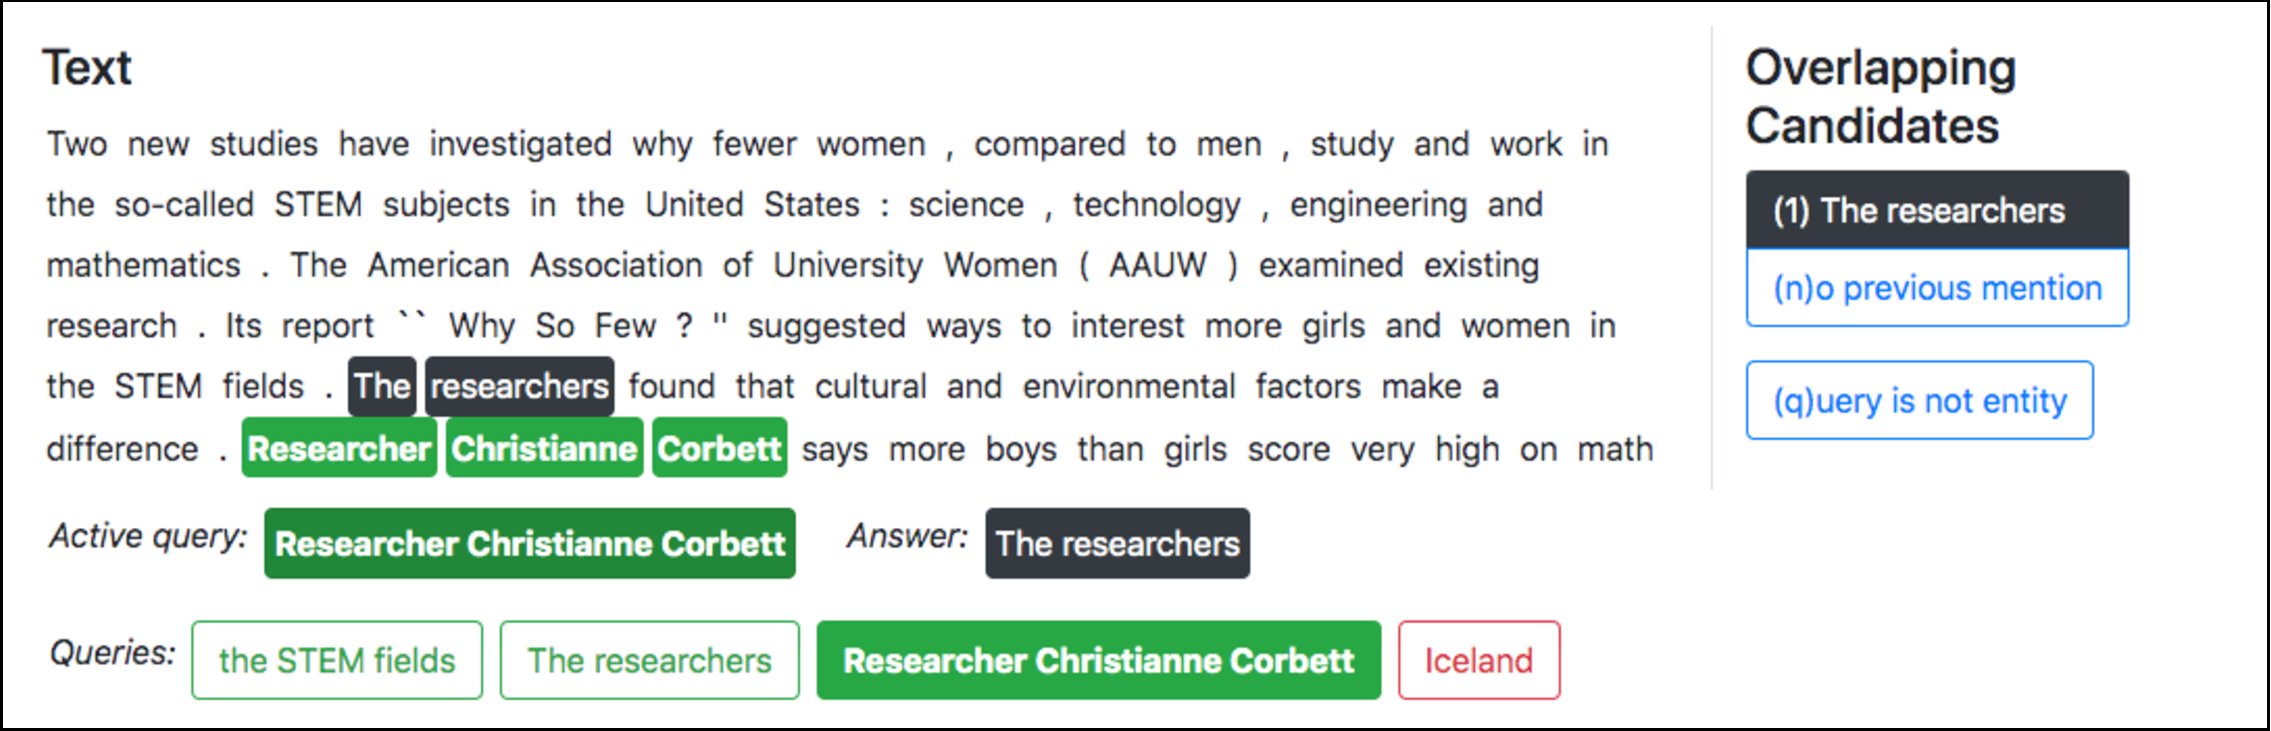
\includegraphics[width=\linewidth]{ui.pdf}
    \caption{On the user interface, the sampled span
    is highlighted and the user must select an antecedent. If
    no antecedents exist or the span is not an entity mention, then the user
    will click the corresponding buttons.
    }
    \label{fig:ui}
\end{figure*}


\begin{figure}[!t]
    \centering
    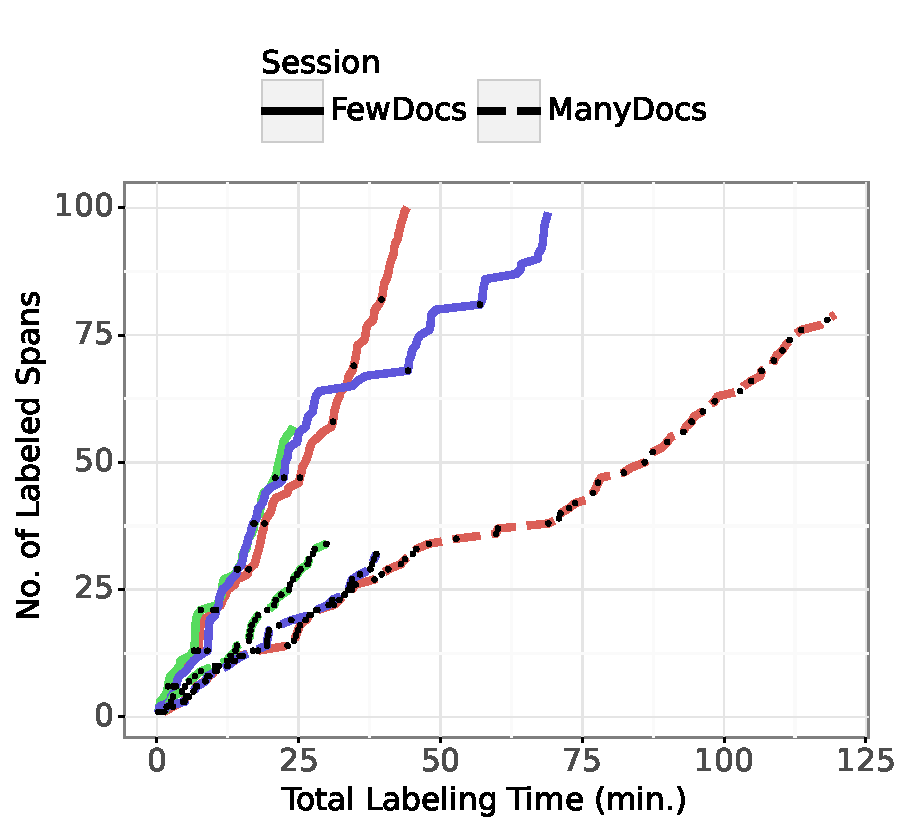
\includegraphics[width=\linewidth]{userstudy_full.pdf}
    \caption{Full annotation times of participants (distinguished by color) during the user study. Over a
    longer period of time, the difference in number of labeled spans between the
    two sessions is much more pronounced. Within fourty-five minutes, the
    {\color{red}red} user can label a
    hundred spans in the \textbf{FewDocs} session but only labels about thirty spans
    in the \textbf{ManyDocs} session.}
    \label{fig:full}
\end{figure}

\subsection{User Study}
\label{ssec:user_appendix}

\paragraph{Instructions to Participants} We give the following instructions
to user study participants:
\begin{displayquote}
\normalsize
You will be shown several sentences from a
document. We have highlighted a mention (a word or phrase) of an entity (a
person, place, or thing). This entity mention may be a pronoun (such as ``she''
or ``their'') or something else. 

We need your help to find an earlier mention of
the same entity, whether in the same sentence or in an earlier sentence. The
mention does not have to be the immediately previous one. 

If the span is not an
entity mention or does not have an antecedent, please make note of it on the
interface.
\end{displayquote}

\paragraph{User Interface} We design a user interface for annotators to label
coreference (Figure~\ref{fig:ui}). The user interface takes the sampled spans from active learning as
input. Afterward, it will present the document and highlight the sampled spans
in the document. The user the proceeds to go through the list of ``Queries''.
For the ``Active query'', they need to either: find its antecedent, mark there
is ``no previous mention'', or indicate that ``query is not an entity''. The
interface will suggest some overlapping candidates to help narrow down the
user's search. The candidates are spans that the \coref{} model scores as likely entity mentions. Users may use keyboard shortcuts to minimize labeling time. The code for the user interface is released along with the code for the simulations.





\paragraph{Extending Annotation Time}


User study participants are asked to annotate at least twenty-five minutes
(Section~\ref{ssec:human_labeling}). During the study, two participants continue to label
after the minimum duration. Figure~\ref{fig:full} shows full results from the
user study. Over a longer duration, the differences between the \textbf{FewDocs}
and \textbf{ManyDocs} sessions are clearer.

\subsection{Examples of Sampled Spans}
\label{ssec:examples}
We provide examples of spans that are sampled from the experiments. For these
examples, we look at the simulation where document reading is constrained to one
document and twenty spans are sampled per cycle. We compare the spans sampled by
each strategy for both \preco{} (Table~\ref{tab:examples_preco}) and \qbcoref{}
(Table~\ref{tab:examples_qbcoref}). Across domains, the strategies behave
similarly, but we notice some differences in \textbf{ment-ent} and
\textbf{joint-ent}.  In \preco{}, those strategies tend to sample a mix of spans
that are and are not entity mentions (Section~\ref{ssec:distribution}).  In \qbcoref{}, they sample more entity
mentions. This could be due to more entity mentions present in a Quizbowl
question, which makes it more likely to sample something that should belong to
an entity cluster.

For other strategies, we notice some issues. As mentioned in Section~\ref{ssec:error}, \textbf{li-clust-ent} tends to
sample nested entity mentions, which may become redundant for annotators to
label. In fact, \avgfone{} for \textbf{li-clust-ent} tends to be lower if
document reading is constrained to one document. \textbf{Cond-ent} suffers from
redundant labeling because pronouns are repeatedly sampled and they tend to
link to the same entity cluster.

\latexfile{examples.tex}

